\documentclass[11pt,fleqn]{article}

%% This first part is the document header, which you don't need to edit.
%% Scroll down to \begin{document}

\usepackage[latin1]{inputenc}
\usepackage{enumerate}
\usepackage[hang,flushmargin]{footmisc}
\usepackage{mdframed}
\usepackage{minted}
\usepackage{color}
\usepackage{datetime}
\usepackage{graphicx}
%%Please place all images used in documents in the images folder
\graphicspath{ {../images/} }
%% USAGE: \includegraphics[args1 = val1, args2 = val2]{filename}
\setlength{\oddsidemargin}{0px}
\setlength{\textwidth}{460px}
\setlength{\voffset}{-1.5cm}
\setlength{\textheight}{20cm}
\setlength{\parindent}{0px}
\setlength{\parskip}{10pt}

\newcommand{\mil}[2][java]{\mintinline{#1}|#2|}
%% This command allows quick use of \mintinline feature, default language is java.

%% USAGE: \mil (optional)[<language>] {content}

%% EXAMPLE: \mil[python]{if not x == 3}
%% 			\mil{if (x.equals(y)}

\begin{document}
\title{Primitive Types and Math}%Insert Title here
\author{Tim Magoun and Aravind Koneru}
\date{\textit{Compiled on} \today \hspace{1mm} at \currenttime}
\maketitle

\begin{abstract}
In this lesson we will set up your computer for Java programming, and learn about some of the primitive types in Java. In the second half of this lesson, we will learn about the simple arithmetic operations that we'll use in the future.
\end{abstract}

\section*{Foreword}
Programming is an ever-increasingly useful skill to have in the digital world. Before learning about the basics of Java, one must realize the following:
\begin{itemize}
\item Programming is the act of writing instructions for a computer
\item The computer could only do one thing at a time
\item Programming is supposed to make repetitive tasks easier
\item It is more important to understand the concept rather than memorizing syntax
\end{itemize}
Feel free to ask questions, they don't have to be about the current exercise.

\newpage
\section{Installing Eclipse}
Just follow the instructions on the course syllabus, which is also included below:
\begin{enumerate}
\item Go to \texttt{https://eclipse.org/downloads/eclipse-packages/}
\item Click on the corresponding installer, 32 bit or 64 bit (if you don't know the version of OS present, choose the 32 bit installer)
\item Download the installer to a known location (ex. Downloads or Desktop)
\item Execute the installer file
\item Select Eclipse IDE for Java Developers
\item Confirm install location and select preferred shortcut locations
\item Accept EULA
\item Bogosort the digits of $\pi$
\item Launch Eclipse Neon and set up preferences, line numbers are highly recommended
\end{enumerate}

\section{Creating a Java Project}
\begin{enumerate}
\item Start up Eclipse and make the workspace in a known location (ex. Documents)
\item Enter into the Java Perspective
\item Right click on \textbf{Package Explorer}, which is on the left part of the screen, and select \textbf{New} $\rightarrow$ \textbf{Java Project}
\item Name the project \textbf{Lesson 1} and click \textbf{Finish}
\end{enumerate}

\section{The Primitive Types}
Create a new class in your \textbf{Lesson 1} project by expanding the project, right click on \textbf{src}, and select \textbf{New} $\rightarrow$ \textbf{Class}. Name your class \textbf{PrimativeTypeExplorer} and select the check-box \textbf{public static void main(String[] args)} under the last large text field, and "Which method stubs would you like to create?"

Your screen should look somewhat like this:

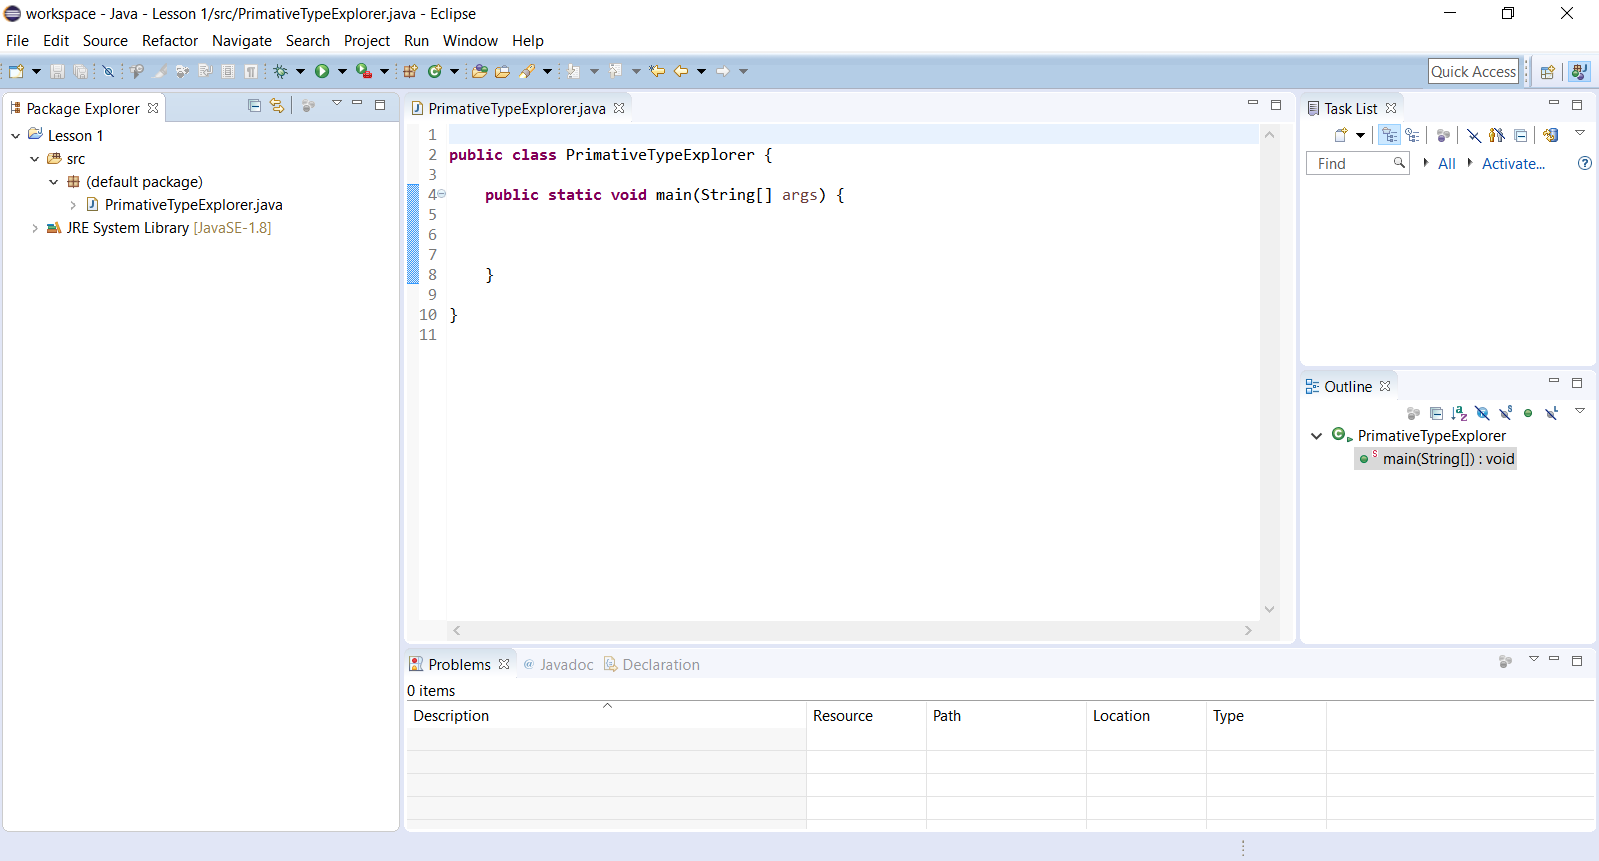
\includegraphics[scale=0.5]{Lesson_1_1.png}



\end{document}
